\documentclass[ignorenonframetext,ucs]{beamer}

\usepackage[ngerman]{babel}
\usepackage{ucs}
\usepackage[utf8x]{inputenc}
\usepackage[T1]{fontenc}
\usepackage{relsize}
\usepackage{lmodern}

\PreloadUnicodePage{0}

%\usepackage[colorlinks]{hyperref}
\newcommand\refurl[2]{#2\footnote{\url{#1}}}

\usepackage{graphicx}
\definecolor{darkgreen}{rgb}{0,0.5,0}
\usetheme[compress]{Berlin}

\title{Unter~dem~Radar~— Das~Zensusgesetz~2011}
\subtitle{All~Your~Database Are~Belong To~Us}
\author{Oliver~„Unicorn“~Knapp \and Tim~„Scytale“~Weber}
\institute{
	Chaos~Computer~Club~e.V. % \and
%	oqlt~e.V. \and
%	RaumZeitLabor~Mannheim
}
\date{22.~Mai~2010\\SIGINT~2010, Köln}

\begin{document}

\frame{\titlepage}

\section{Einführung}

%\subsection{Die Referenten}

\subsection{Der Zensus, das unbekannte Wesen}

\begin{frame}{Was ist ein Zensus?}\begin{itemize}
\item Volkszählung, Zensus, Census
\item mehr als nur Zählen
\item Makrozensus: alle werden gezählt
\item Mikrozensus: repräsentative Stichproben
\item Durchführungsarten:\begin{itemize}
	\item „klassischer“ Zensus: Umfragebögen
	\item Registerzensus: keine Umfragen, sondern Melderegister
	\item registergestützter Zensus: Mischform;\\Melderegister ergänzt durch Umfragen
\end{itemize}
\end{itemize}\end{frame}

\begin{frame}{Warum das Ganze?}\begin{itemize}
\item Bevölkerungszusammensetzung und -verteilung
\item Planung (Wohnungsbau, Infrastruktur, …)
\item Finanzierung (Steuerschätzung, Länderfinanzausgleich,\\kommunale Haushalte, …)
\item Bildungsniveau, Ausländeranteil, Religionszugehörigkeit, Familienstruktur, …)
\end{itemize}\end{frame}

\subsection{Geschichte der Volkszählungen}

\begin{frame}{Im Nationalsozialismus}\begin{itemize}
\item 1933, 1939; Volks-, Berufs-, Betriebszählungen
\item Erfassung von „Glaubens-“ und „Geltungsjuden“\\sowie „Mischlingen“
\item Name, Geburtsname, Religion, Muttersprache,\\Volkszugehörigkeit, Beruf
\item Verwandschaftsbeziehung
\end{itemize}\end{frame}

\begin{frame}{In der DDR}\begin{itemize}
\item 1950 und 1964 Volks- und Berufszählungen
\item 1971 und 1981 Volks-, Berufs-, Wohnraum-\\und Gebäudezählungen
\item Ergebnisse aus politischen Gründen\\teilweise nicht veröffentlicht
\end{itemize}\end{frame}

\begin{frame}{In der Bundesrepublik}\begin{itemize}
\item 1961 und 1970 Volks- Berufs- und Arbeitsstättenzählungen
\item 1950 und 1987 Volks-, Berufs-, Gebäude-, Wohnungs-\\und Arbeitsstättenzählungen
\item Volkszählung egtl. für 1981 geplant\begin{itemize}
	\item Finanzierungsstreit, Gesetz erst 1982 verabschiedet
	\item Zähltermin daher 1983
	\item 500~Verfassungsklagen, Änderungsbedarf
	\item verschoben bis 1987
\end{itemize}
\end{itemize}\end{frame}

\subsection{Die Volkszählung 1983/87}

\begin{frame}{Argumente der Gegner}\begin{itemize}
\item Zwangsbefragung (Bußgeld bis 10.000~Mark)
\item Rechtsweg abgeschnitten (keine aufschiebende Wirkung)
\item „rosa Listen“, Anstaltsinsassen
\item keine Anonymität, Melderegisterrückfluss
\item Kopfprämien (2,50~Mark für nicht Gemeldete,\\5~Mark für nicht gemeldete Ausländer)
\item Übergröße gegen Postversand, nicht knicken
\item Zähler im eigenen Wohnbezirk
\end{itemize}\end{frame}

\begin{frame}{Ziviler Ungehorsam}\begin{itemize}
\item Ausfüllen mit Kuli (Graphitleser)
\item falsche Zähler sammeln Bögen ein
\item handschriftlicher Lebenslauf
\item abschneiden der Kennnummer
\item Falschangaben
\end{itemize}\end{frame}

\begin{frame}{Volkszählungsurteil}\begin{itemize}
\item informationelle Selbstbestimmung: \emph{Wer unsicher ist, ob abweichende Verhaltensweisen jederzeit notiert und als Information dauerhaft gespeichert, verwendet oder weitergegeben werden, wird versuchen, nicht durch solche Verhaltensweisen aufzufallen.}
\end{itemize}\end{frame}

\begin{frame}{Zur „Ordnungsnummer“}
\emph{\scriptsize Das Erhebungsprogramm vermag zwar einzelne Lebensbereiche, zum Beispiel den Wohnbereich des Bürgers, jedoch nicht dessen Persönlichkeit abzubilden. Etwas anderes würde nur gelten, soweit eine unbeschränkte Verknüpfung der erhobenen Daten mit den bei den Verwaltungsbehörden vorhandenen, zum Teil sehr sensitiven Datenbeständen oder gar die Erschließung eines derartigen Datenverbundes durch ein einheitliches Personenkennzeichen oder sonstiges Ordnungsmerkmal möglich wäre; denn eine umfassende Registrierung und Katalogisierung der Persönlichkeit durch die Zusammenführung einzelner Lebensdaten und Personaldaten zur Erstellung von Persönlichkeitsprofilen der Bürger ist auch in der Anonymität statistischer Erhebungen unzulässig. Derartigen Datenverbindungen - Totalabbildern - steht schon § 11 BStatG entgegen, der sogar die Übermittlung von nicht anonymisierten Einzelangaben zwischen den mit der Durchführung einer Bundesstatistik betrauten Personen und Stellen nur erlaubt, soweit dies zur Erstellung der Bundesstatistik erforderlich ist.}
\end{frame}

\subsection{Volkszählungen nach der Wiedervereinigung}

\begin{frame}{Deutsche Volkszählung 1991}\begin{itemize}
\item angedacht wegen Wiedervereinigung
\item nicht durchgeführt:\begin{itemize}
	\item finanzielle Gründe
	\item Ablehnung in Politik und Bevölkerung
\end{itemize}
\end{itemize}\end{frame}

\begin{frame}{EU-Zensusrunde 2000/2001}\begin{itemize}
\item ohne Schweden und Deutschland
\item deutsches Argument: Ablehnung bei Bevölkerung
\end{itemize}
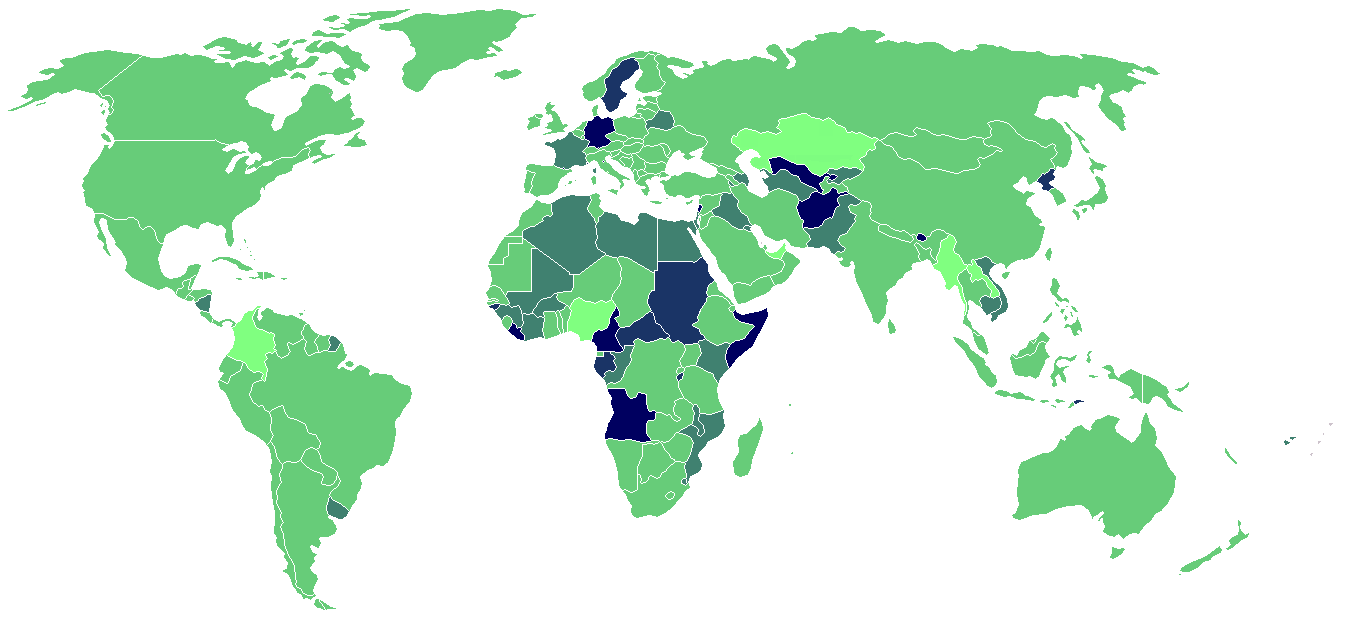
\includegraphics[height=4cm]{most-recent-census.png}
\end{frame}

\begin{frame}{Steuernummer 2007}\begin{itemize}
\item im Prinzip Registerzensus (Meldedaten)
\item bundesweite Personenkennziffer
\item Rückfluss an die Meldeämter
\item keine Verwendung für Statistik
\item Klage ist wohl vergessen worden
\end{itemize}\end{frame}

\section{Volkszählung 2011}

\subsection{Alles Gute kommt aus Brüssel}

\begin{frame}{Der EU-Beschluss}\begin{itemize}
\item Bundesregierung entscheidet August 2006:\\Deutschland macht mit
\item EU-Verordnung 763/2008, 9. Juli 2008
\item verschiedene Zählarten möglich\\(kein Zwang zum registergestützten)
\end{itemize}\end{frame}

\subsection{Das Bundesgesetz}

\begin{frame}{Was sagt das Bundesgesetz?}\begin{itemize}
\item „Gesetz über den registergestützten Zensus\\im Jahr 2011„ (ZensG 2011)
\item Inkrafttreten am 16. Juli 2009
\item Zusammenführen der Daten von\begin{itemize}
	\item Meldeämtern
	\item Bundesagentur für Arbeit
	\item „Personalbehörden“ (Beamte)
\end{itemize} bei den Landesstatistikämtern,\\dann an Bundesstatistikamt
\end{itemize}\end{frame}

\begin{frame}{Kritische Stellen}\begin{itemize}
\item keine Anonymisierung
\item Religionszugehörigkeit
\item Migrationshintergrund
\item Daten von Meldeämtern und BA zweckentfremdet
\item Zwangsverpflichtung zur Auskunft (sonst Bußgeld)
\item Übertragung der Übermittlungssperre (mit Grund)
\item „Sonderbereiche“
\item Datensicherheit
\end{itemize}\end{frame}

\begin{frame}{Personenkennziffer}\begin{itemize}
\item \emph{Für jede Anschrift, jedes Gebäude, jede Wohnung, jeden Haushalt und jede Person wird von den statistischen Ämtern des Bundes und der Länder eine Ordnungsnummer vergeben und geführt, die gemeinde- und gebäudeübergreifend sein kann. Die Ordnungsnummern dürfen bei den Zusammenführungen nach §~9 verwendet werden.}
\end{itemize}\end{frame}

\begin{frame}{Rückfluss der Daten}\begin{itemize}
\item \emph{Für die Verwendung gegenüber den gesetzgebenden Körperschaften und für Zwecke der Planung, jedoch nicht für die Regelung von Einzelfällen, dürfen die statistischen Ämter des Bundes und der Länder den obersten Bundes- oder Landesbehörden Tabellen mit statistischen Ergebnissen übermitteln, auch soweit Tabellenfelder nur einen einzigen Fall ausweisen.}
\end{itemize}\end{frame}

\subsection{Umsetzung in den Ländern}

\begin{frame}{Anfrage Hessen}\begin{itemize}
\item mündliche Anhörung, bestritten durch Unicorn
\item Beschlussnahme direkt nach Anhörung
\item Abschottungsgrundsatz
\end{itemize}\end{frame}

\begin{frame}{Anfrage Thüringen}\begin{itemize}
\item schriftliche Anhörung (ergo: Text verfassen)
\item bessere Abschottung
\item Datenübertragung via DOI
\end{itemize}\end{frame}

\section{Nächste Schritte}

\subsection{Liebesgrüße aus Karlsruhe}

\begin{frame}{Verfassungsklage}\begin{itemize}
\item Stichtag 16. Juli 2010 (1-Jahres-Frist)
\item bislang klagt noch niemand(!)
\item wer will?
\item Grüne haben 1983 protestiert,\\verhalten sich jetzt aber ruhig
\item Linke sind eher dagegen
\item „die üblichen Verdächtigen“ müssen wohl ran
\end{itemize}\end{frame}

\begin{frame}{Argumente für die Klage}\begin{itemize}
\item informationelle Selbstbestimmung?
\item mehr als EU-Richtlinie (Religion)
\item bundeseinheitliche Personenkennziffer (Primärschlüssel)
\item fehlende Anonymisierung
\item umfassendes Personenprofil
\end{itemize}\end{frame}

\subsection{Tell a friend!}

\begin{frame}{Bevölkerung informieren}\begin{itemize}
\item Freunde, Familie, Aktivisten
\item Blogbeiträge
\item bei Presse und Rundfunk anfragen
\item Aktionen, Flyer, Aufkleber
\item you name it!
\end{itemize}\end{frame}

\end{document}
